\documentclass[8pt]{beamer}
\usepackage[utf8]{inputenc}
\usepackage{ulem}
\usepackage{xcolor}
\usepackage{colortbl}
\usepackage{epsfig}
% \usepackage{cancel}
\usepackage{ulem}
% \usepackage{threeparttable} % Joao Pela: 
\usepackage{amsmath}
\usepackage{hyperref}
\usepackage{appendixnumberbeamer}
\usepackage{pdfpages}
% \usepackage{feynmp}         % For latex produced Feynman Diagrams

% Rule for feynmp diagrams to be considered graphics
% \DeclareGraphicsRule{*}{mps}{*}{}
% 
% % New compile sequence for feynmp
% \makeatletter
% \def\endfmffile{%
%   \fmfcmd{\p@rcent\space the end.^^J%
%           end.^^J%
%           endinput;}%
%   \if@fmfio
%     \immediate\closeout\@outfmf
%   \fi
%   \ifnum\pdfshellescape=\@ne
%     \immediate\write18{mpost \thefmffile}%
%   \fi}
% \makeatother

\usetheme{Madrid}

\author[J. Pela]{J. Pela}
\title{Study on Tracks Information}
\institute[ICL]{Imperial College London}
\date{2014-06-03}

% The log drawn in the upper right corner.
\logo{\includegraphics[height=0.115\paperheight]{img/Logo_CMSICL.png}}

\begin{document}
\setlength{\unitlength}{1mm}

% ###################################################
\begin{frame}
  \titlepage
\end{frame}

% ###################################################
\begin{frame}{Today's presentation}
 
\begin{block}{Topics}
 
\begin{itemize}
  \item Preliminary study on the new variables using tracking information
\end{itemize}

\end{block}

\end{frame}

% ###################################################
\begin{frame}{Motivation}

In our signal there is no colour connection between the VBF jets, this is the motivation for the Central Jet Veto.

\begin{block}{CJV Definition}

Veto an event if there is a jet:
\begin{itemize}
  \item Between both selected jets
  \item Minimum jet $p_T > 30$ GeV passing PU ID
\end{itemize}

\end{block}

\begin{block}{CJV Disadvantages}
 
\begin{itemize}
  \item Assumes colours connection will manifest as reconstructed jets
  \item Minimum $p_T$ 
  \item Only looks for objects between the 2 selected jets.
\end{itemize}

\end{block}

So I suggest as a complementary variable(s) look at the tracking information.

\end{frame}

% ###################################################
\begin{frame}{Definition}
 
For our signal if we assume we selected the correct primary vertex:
\begin{block}{Reasoning}
 
\begin{itemize}
  \item Tracks coming out of this vertex should be just our jets and the underlying event.
  \item Therefore most tracks above a minimum $p_T$ threshold should be in our jets.
  \item This should not be true for our background since colour connection implies presence of particles and/or jets on the event coming from the primary vertex.
  \item We can define/study variables to look at the this difference between signal and background.
\end{itemize}

CAVEAT: The assumption of correct primary vertex be an incorrect if both signal jets are outside the tracking region
 
\end{block}
 
\begin{block}{Definition} 

Select events where the 2 leading jets:
\begin{itemize}
  \item $p_T<50$ and $|\eta|<4.7$
  \item Pass PU ID
\end{itemize}

Look at:
\begin{itemize}
  \item Ratio of number track outside jets
  \item Ratio of track energy outside jets
\end{itemize}

We can also compare this to current CJV cut

\end{block}

\end{frame}




% ###################################################
\begin{frame}{Tracks $p_T>0$ - All events}

All Plots from now on, signal (red) and VBF QCD (green). All plots scaled to 1. Y-axis covers $[0,1[$ (to be fixed later).

\begin{columns}
 
\column[t]{0.45\linewidth}
\begin{block}{Outside Number Ratio}
 
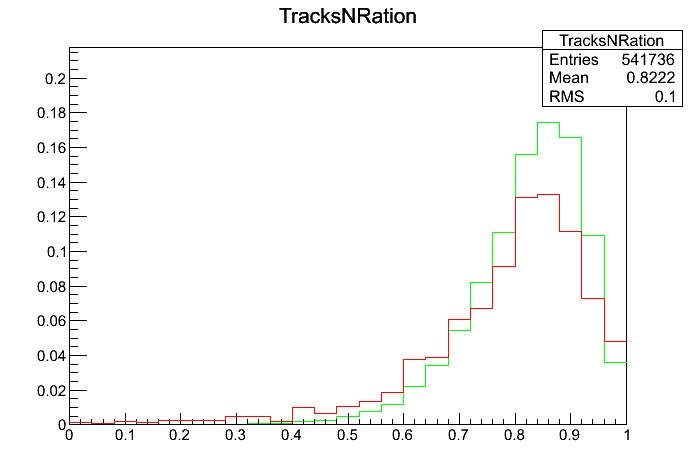
\includegraphics[width=\linewidth]{img/Tracks0_TracksNRatio.png}

\end{block}

\column[t]{0.45\linewidth}
\begin{block}{Outside Energy Ratio}
 
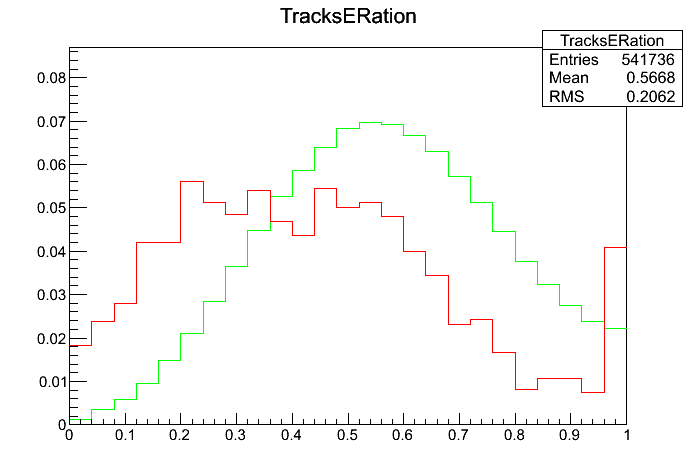
\includegraphics[width=\linewidth]{img/Tracks0_TracksERatio.png}
 
\end{block}

\end{columns}

\end{frame}

% ###################################################
\begin{frame}{Tracks $p_T>1$ - All events}

\begin{columns}
 
\column[t]{0.45\linewidth}
\begin{block}{Outside Number Ratio}
 
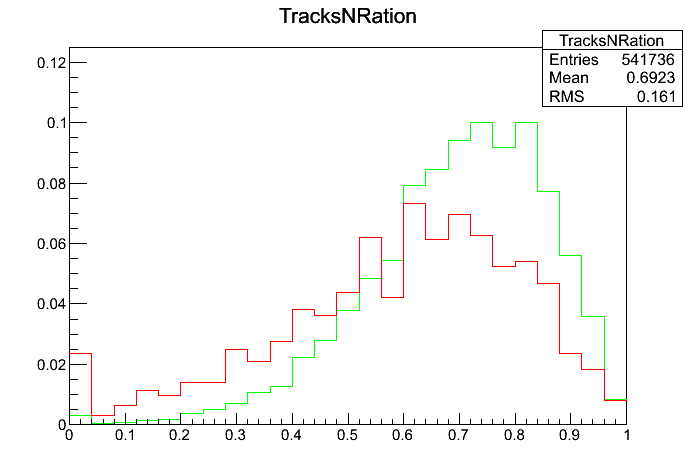
\includegraphics[width=\linewidth]{img/Tracks1_TracksNRatio.png}

\end{block}

\column[t]{0.45\linewidth}
\begin{block}{Outside Energy Ratio}
 
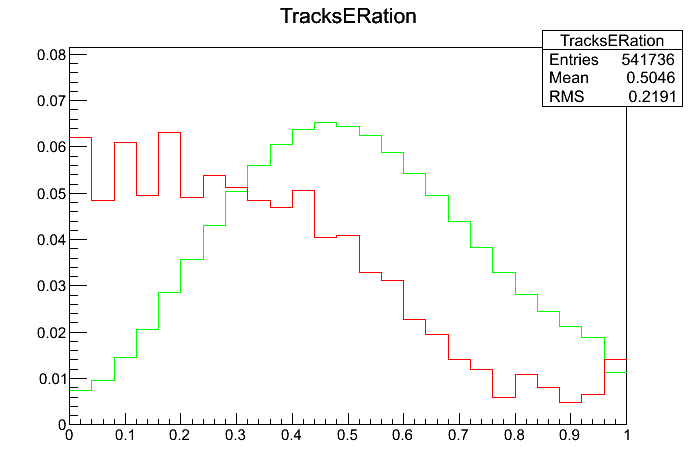
\includegraphics[width=\linewidth]{img/Tracks1_TracksERatio.png}
 
\end{block}

\end{columns}

\end{frame}

% ###################################################
\begin{frame}{Tracks $p_T>2$ - All events}

\begin{columns}
 
\column[t]{0.45\linewidth}
\begin{block}{Outside Number Ratio}
 
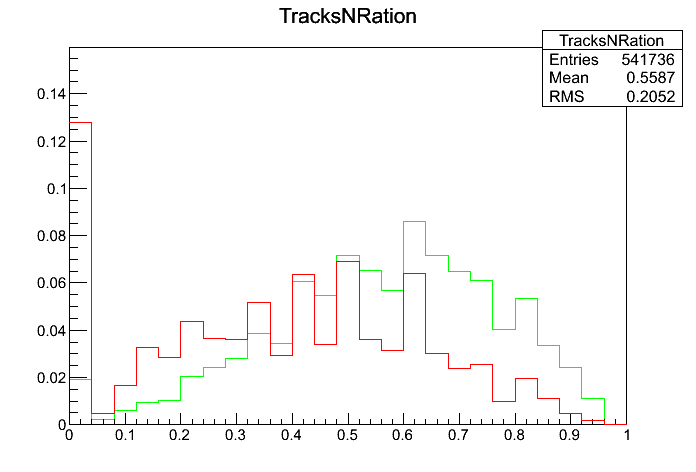
\includegraphics[width=\linewidth]{img/Tracks2_TracksNRatio.png}

\end{block}

\column[t]{0.45\linewidth}
\begin{block}{Outside Energy Ratio}
 
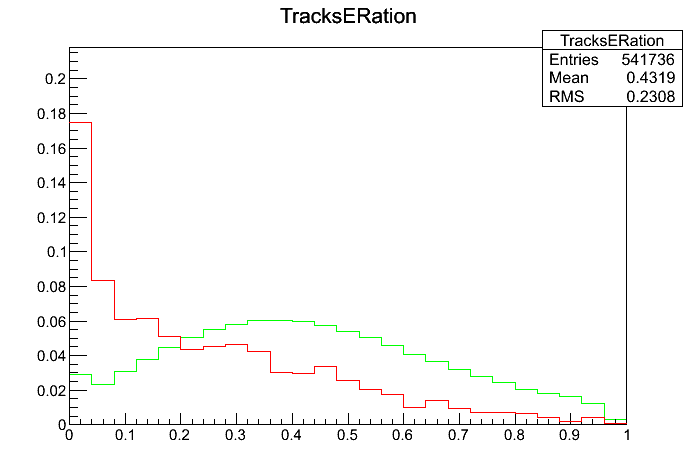
\includegraphics[width=\linewidth]{img/Tracks2_TracksERatio.png}
 
\end{block}

\end{columns}

\end{frame}

% ###################################################
\begin{frame}{Tracks $p_T>1$ - All events CJV Pass}

\begin{columns}
 
\column[t]{0.45\linewidth}
\begin{block}{Outside Number Ratio}
 
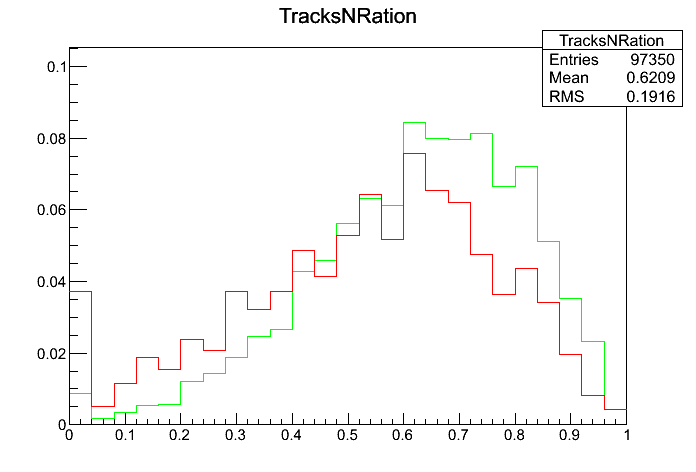
\includegraphics[width=\linewidth]{img/Tracks1_CJVPass_TracksNRation.png}

\end{block}

\column[t]{0.45\linewidth}
\begin{block}{Outside Energy Ratio}
 
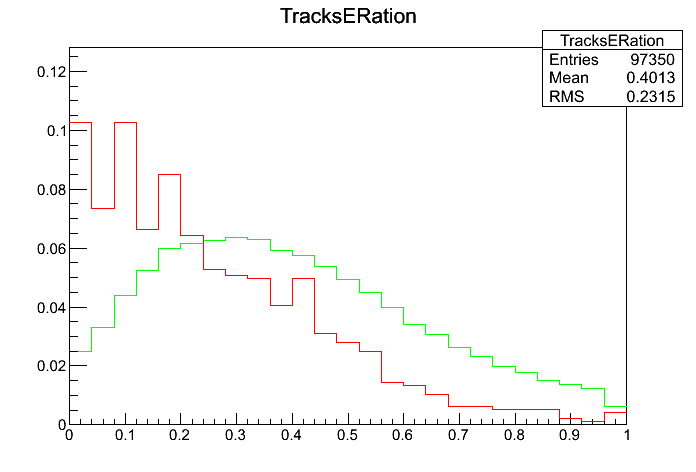
\includegraphics[width=\linewidth]{img/Tracks1_CJVPass_TracksERation.png}
 
\end{block}

\end{columns}

\end{frame}

% ###################################################
\begin{frame}{Tracks $p_T>1$ - BB}

\begin{columns}
 
\column[t]{0.45\linewidth}
\begin{block}{Outside Number Ratio}
 
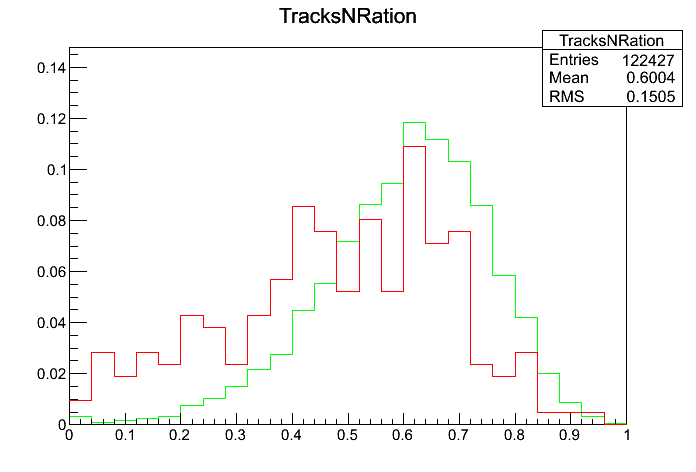
\includegraphics[width=\linewidth]{img/BB_Tracks1_TracksNRatio.png}

\end{block}

\column[t]{0.45\linewidth}
\begin{block}{Outside Energy Ratio}
 
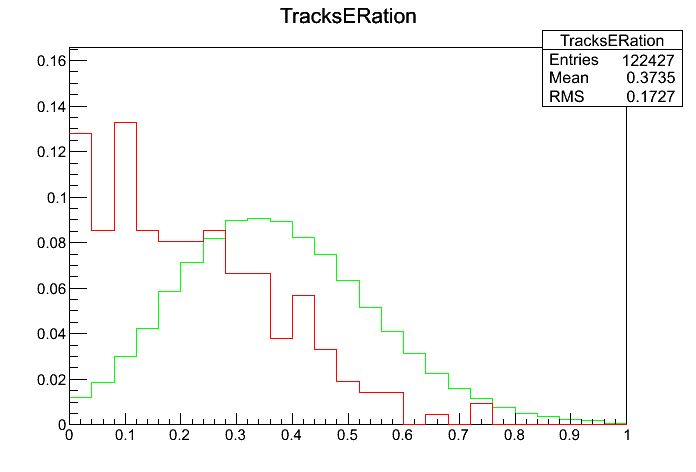
\includegraphics[width=\linewidth]{img/BB_Tracks1_TracksERatio.png}
 
\end{block}

\end{columns}

\end{frame}

% ###################################################
\begin{frame}{Tracks $p_T>1$ - BE}

\begin{columns}
 
\column[t]{0.45\linewidth}
\begin{block}{Outside Number Ratio}
 
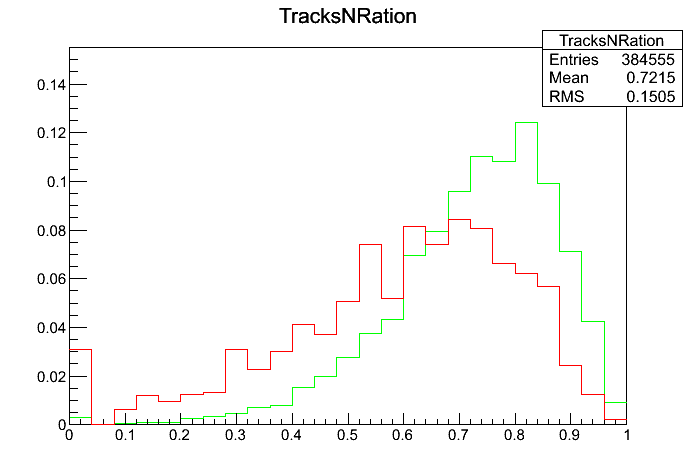
\includegraphics[width=\linewidth]{img/BE_Tracks1_TracksNRatio.png}

\end{block}

\column[t]{0.45\linewidth}
\begin{block}{Outside Energy Ratio}
 
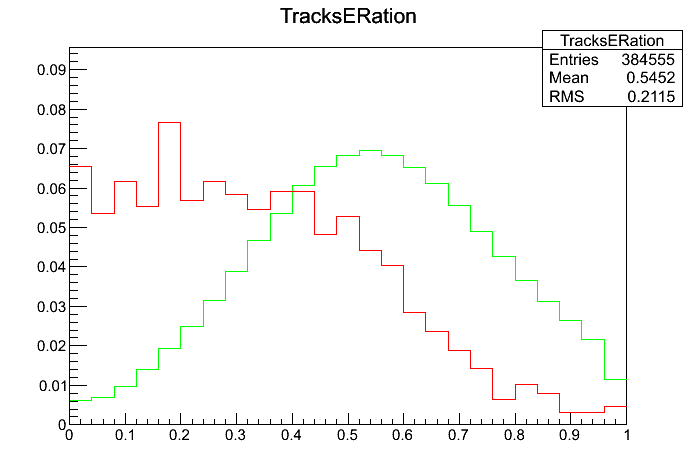
\includegraphics[width=\linewidth]{img/BE_Tracks1_TracksERatio.png}
 
\end{block}

\end{columns}

\end{frame}

% ###################################################
\begin{frame}{Tracks $p_T>1$ - EE}

\begin{columns}
 
\column[t]{0.45\linewidth}
\begin{block}{Outside Number Ratio}
 
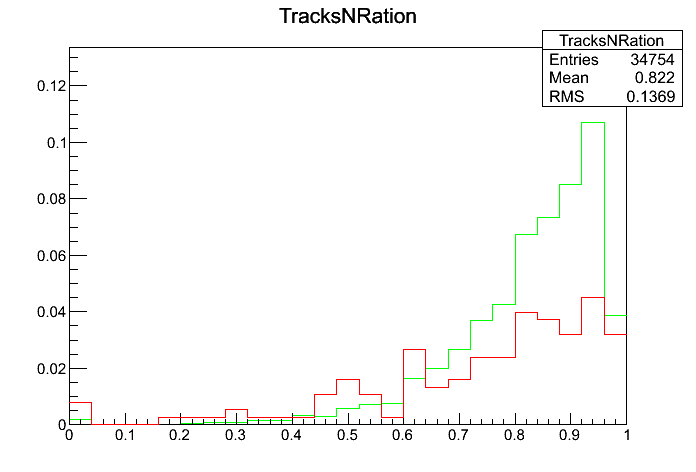
\includegraphics[width=\linewidth]{img/EE_Tracks1_TracksNRatio.png}

\end{block}

\column[t]{0.45\linewidth}
\begin{block}{Outside Energy Ratio}
 
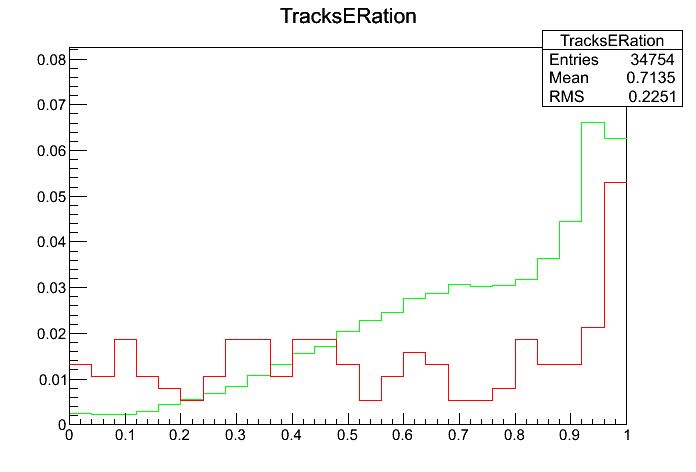
\includegraphics[width=\linewidth]{img/EE_Tracks1_TracksERatio.png}
 
\end{block}

\end{columns}

\end{frame}

% ###################################################
\begin{frame}{Summary and next steps}
 
\begin{block}{Summary:}
 
\begin{itemize}
  \item Energy ration is a descriminat variable that add information to CJV
\end{itemize}

\end{block}

\begin{block}{Next Steps:}
 
\begin{itemize}
  \item Study including this variables in our mva.
  \item MVA optimization
  \item L1-HLT studies
\end{itemize}
 
\end{block}

\end{frame}


% ###################################################
\appendix
% ###################################################
\begin{frame}
 
\begin{block}

\begin{center}Backup Slides\end{center}

\end{block}

\end{frame}

% {
% \setbeamercolor{background canvas}{bg=}
% \includepdf[pages=11]{hinv_magnan_140506.pdf}
% }

\end{document}